% This file was converted to LaTeX by Writer2LaTeX ver. 1.4
% see http://writer2latex.sourceforge.net for more info
\documentclass[a4paper]{article}
\usepackage[utf8]{inputenc}
\usepackage[T2A,T1]{fontenc}
\usepackage[russian,english]{babel}
\usepackage{amsmath}
\usepackage{amssymb,amsfonts,textcomp}
\usepackage{color}
\usepackage{array}
\usepackage{supertabular}
\usepackage{hhline}
\usepackage{hyperref}
\hypersetup{pdftex, colorlinks=true, linkcolor=blue, citecolor=blue, filecolor=blue, urlcolor=blue, pdftitle=\textcyrillic{Станс 1 (Сыкун-ту)     }}
\usepackage[pdftex]{graphicx}
% Outline numbering
\setcounter{secnumdepth}{0}
\makeatletter
\newcommand\arraybslash{\let\\\@arraycr}
\makeatother
% Page layout (geometry)
\setlength\voffset{-1in}
\setlength\hoffset{-1in}
\setlength\topmargin{0.4925in}
\setlength\oddsidemargin{0.5909in}
\setlength\textheight{10.254965in}
\setlength\textwidth{7.087in}
\setlength\footskip{16.3056pt}
\setlength\headheight{12pt}
\setlength\headsep{0.0598in}
% Footnote rule
\setlength{\skip\footins}{0.0469in}
\renewcommand\footnoterule{\vspace*{-0.0071in}\setlength\leftskip{0pt}\setlength\rightskip{0pt plus 1fil}\noindent\textcolor{black}{\rule{0.25\columnwidth}{0.0071in}}\vspace*{0.0398in}}
% Pages styles
\makeatletter
\newcommand\ps@Standard{
  \renewcommand\@oddhead{\textstylePageNumber{\textcyrillic{Восток 5}}}
  \renewcommand\@evenhead{\@oddhead}
  \renewcommand\@oddfoot{[Warning: Draw object ignored]}
  \renewcommand\@evenfoot{\@oddfoot}
  \renewcommand\thepage{\arabic{page}}
}
\makeatother
\pagestyle{Standard}
\setlength\tabcolsep{1mm}
\renewcommand\arraystretch{1.3}
\title{\textcyrillic{Станс 1 (Сыкун-ту)     }}
\begin{document}
\clearpage\setcounter{page}{1}\pagestyle{Standard}

\bigskip

\begin{flushleft}
\tablefirsthead{}
\tablehead{}
\tabletail{}
\tablelasttail{}
\begin{supertabular}{|m{1.3712599in}m{2.6712599in}m{2.55316in}|}
\hline
\multicolumn{3}{|m{6.7531595in}|}{{\selectlanguage{russian}\bfseries Станс 1 (Сыкун-ту) \ \ \ \ }

{\selectlanguage{russian} Слева от иероглифов - номера стихов с 1 по 6. Ниже дан построчный перевод. В конце дан
пословный перевод первой строки. Еще ниже — \textit{перевод-парафраз} и пересказ (европейский прозаический). Заголовок
и его переводы опущены.}

~
}\\\hline
\multicolumn{3}{|m{6.7531595in}|}{ 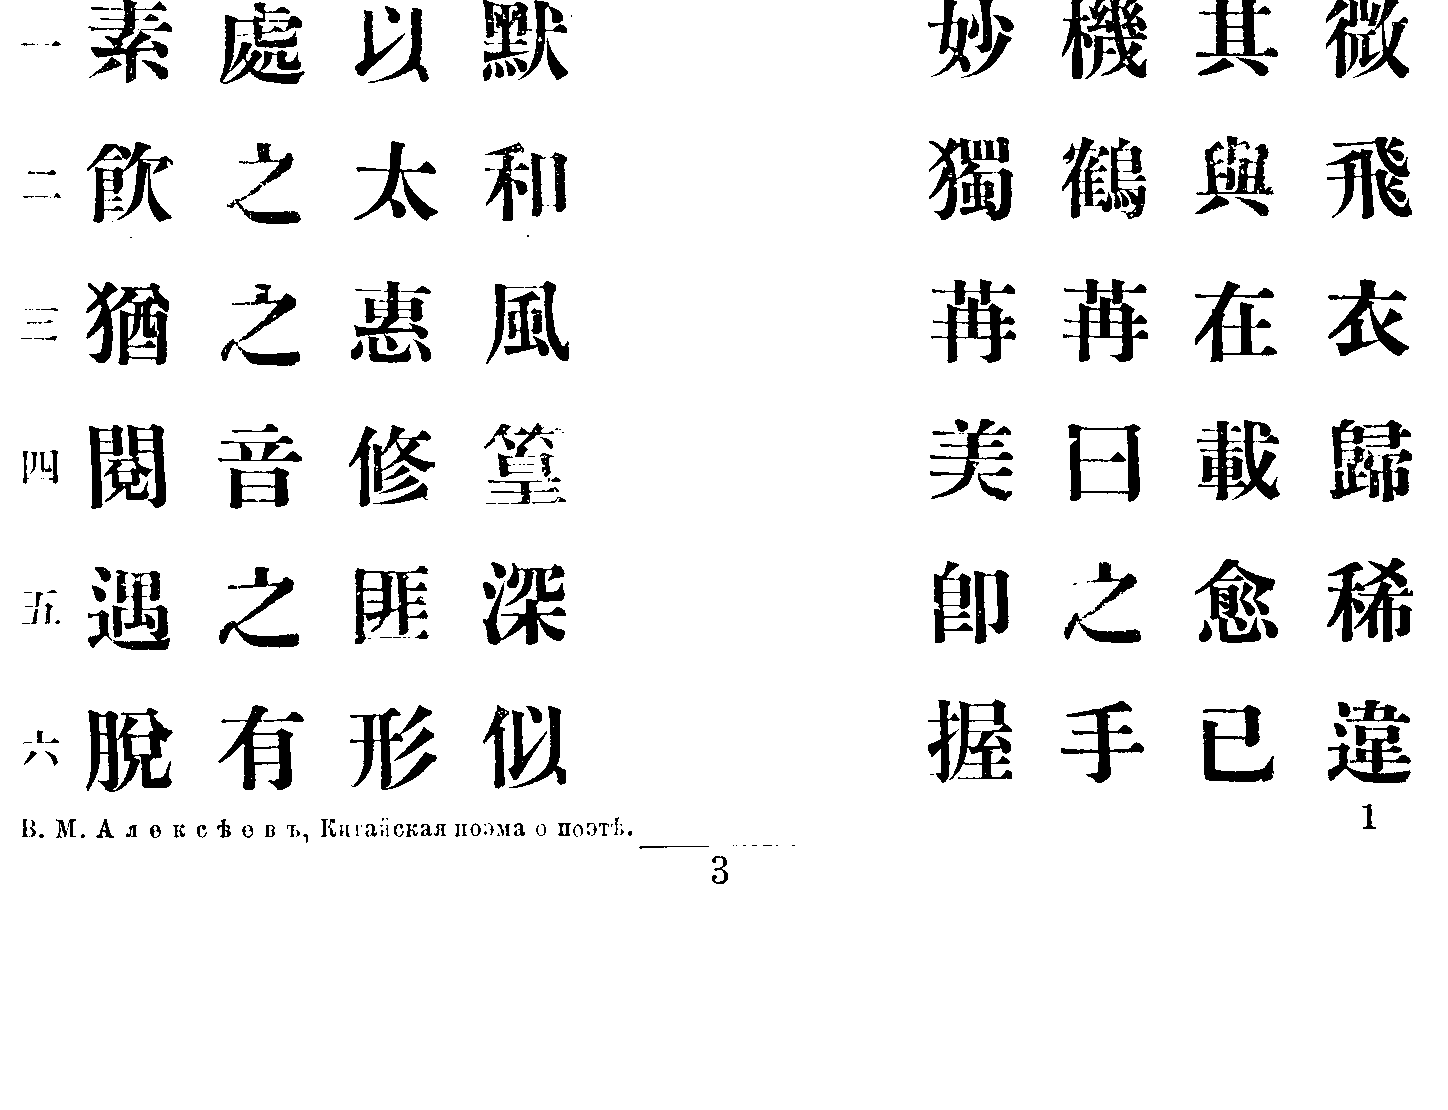
\includegraphics[width=6.25in,height=2.6929in]{A2-img001.png} }\\\hline
 &
 &
\\
 &
 &
\\
 &
 &
\\
 &
 &
\\
 &
 &
\\\hline
\multicolumn{3}{|m{6.7531595in}|}{{\selectlanguage{russian} 1. Великое проявление внешне блекнет, истинная суть внутри
заполняет.}}\\\hline
\multicolumn{3}{|m{6.7531595in}|}{{\selectlanguage{russian} 2. Уходит к пустоте. Входит в хаос. Копит сильное. Делает
мощное.}}\\\hline
\multicolumn{3}{|m{6.7531595in}|}{{\selectlanguage{russian} 3. Полнотою уготовал мириады вещей, прорезает насквозь
величайшие пустыни,}}\\\hline
\multicolumn{3}{|m{6.7531595in}|}{{\selectlanguage{russian} 4. Грудами, грудами масло-тучи, бурный, бурный долгий
ветер.}}\\\hline
\multicolumn{3}{|m{6.7531595in}|}{{\selectlanguage{russian} 5. Преходит ко вне-формам, добывает этот
{\textquotedbl}центр кольца{\textquotedbl}.}}\\\hline
\multicolumn{3}{|m{6.7531595in}|}{{\selectlanguage{russian} 6. Держит оное, не напрягаясь; привлекает оное без
конца.}}\\\hline
\multicolumn{1}{|m{1.3712599in}|}{{\selectlanguage{russian} Пословный перевод строки 1:}} &
\multicolumn{1}{m{2.6712599in}|}{{\selectlanguage{russian}\itshape да \ \ юн \ \ вай \ \ фэй \ \ \ }

{\selectlanguage{russian} Великое \ проявление \ вне \ \ изменяется\textit{ }}} &
{\selectlanguage{russian} \textit{чжэнь \ \ ти \ \ \ нэй \ \ \ \ чун}\newline
истинная \ \ суть \ \ внутри \ \ заполняет}\\\hline
\end{supertabular}
\end{flushleft}
{\selectlanguage{russian}
Построчный перевод станса:}

\begin{flushleft}
\tablefirsthead{}
\tablehead{}
\tabletail{}
\tablelasttail{}
\begin{supertabular}{|m{0.14765984in}|m{6.34836in}|}
\hline
{\selectlanguage{russian} 1} &
{\selectlanguage{russian} Поэт мощно проявляет себя, но внешне — блекло, а истинная жизнь его всей полнотой в
душе.}\\\hline
{\selectlanguage{russian} 2} &
{\selectlanguage{russian} Поэт уходит духом в емкую пустотность и входит в состояние всеобъемлющести,\newline
он нагромождает в себе все сильное и превращает его в мощное.}\\\hline
{\selectlanguage{russian} 3} &
{\selectlanguage{russian} Поэт держит в себе полностью всю природу, но гением своим прорезает величайшие небесные
пустыни.}\\\hline
{\selectlanguage{russian} 4} &
{\selectlanguage{russian} Таковы огромные тьмы жирных туч, такова дико-свободная, долгая буря.}\\\hline
{\selectlanguage{russian} 5} &
{\selectlanguage{russian} Поэт преходит грани и парит над формами мира: он внедряет в себя абсолютный центр
(Дао).}\\\hline
{\selectlanguage{russian} 6} &
{\selectlanguage{russian} Держать в себе этот мощный дух поэту можно вне усилий, и привлекает он к себе всеобъемлющесть
вне границ.}\\\hline
\end{supertabular}
\end{flushleft}
\subsection[И \ европец промолвил слово:]{И \ европец промолвил слово:}
{\selectlanguage{english}
\foreignlanguage{russian}{\ \ \ \ \ Мощная энергия гения есть лишь внешний фазис его полнозвучной природы.
Всеобъемлющесть духа — вот фонд, из которого как законнейшее и естественнейшее явление вырывается бурным потоком его
натиск в небо. В этом динамическом проявлении своего необъятного духа поэт {\textquotedbl}копит сильное до
мощного{\textquotedbl}, {\textquotedbl}разрезает{\textquotedbl} небо, как дикий вихрь, и пребывает в этом бурном
истечении энергии без усилий, без самоподъема и искусственного напряжения. Эта его динамическая исступленность есть
лишь взрыв накопившейся энергии, {\textquotedbl}сути{\textquotedbl}, заполняющей его душу; есть лишь естественный,
непосредственный порыв мощного духа, которому {\textquotedbl}возвращена емкость{\textquotedbl} и который, очистившись
от прилипаний и осадков жизни, {\textquotedbl}входит во всеобъемлющесть{\textquotedbl}. {\textquotedbl}Держа в себе всю
природу{\textquotedbl}, охватывая собою все, как тяжелые, {\textquotedbl}маслянистые{\textquotedbl} тучи небо, поэт
{\textquotedbl}парит вне форм{\textquotedbl} и навевает на себя полнозвучную
{\textquotedbl}всеобъмлющесть{\textquotedbl} вне всякой меры и предела. Таким образом, в душе поэта есть неиссякаемый,
вечный, всеобъемлющий, как мироздание, источник, из которого бьет фонтан вдохновенной, смелой, не знающей удержу
силы.}}


\bigskip

{\selectlanguage{english}
\foreignlanguage{russian}{Научный анализ Станса 1 — иероглиф за иероглифом, стих за стихом, мысль за мыслью \ — в
неторопливой уважительной полемике с авторитетными знатоками, переводчиками и авторами словарей — не может быть помещен
в наши {\textquotedbl}Тексты{\textquotedbl} (и в наши головы…) как по объему, так и по глубине \newline
(всего 22 страницы, но: объем }\foreignlanguage{russian}{\textbf{${\neq}$}}\foreignlanguage{russian}{ ширина
}\foreignlanguage{russian}{\textbf{х}}\foreignlanguage{russian}{ высота
}\foreignlanguage{russian}{\textbf{х}}\foreignlanguage{russian}{ глубина). }}


\bigskip

\begin{flushleft}
\tablefirsthead{}
\tablehead{}
\tabletail{}
\tablelasttail{}
\begin{supertabular}{|m{0.9045598in}|m{6.01086in}|m{0.09415985in}|}
\hline
{\selectlanguage{russian}\sffamily\color[rgb]{0.2,0.2,0.2} \textlatin{[597D?]}} &
{\selectlanguage{russian} \textsf{\textbf{\textcolor[rgb]{0.2,0.2,0.2}{Значение иероглифа на
русском:}}}\textsf{\textcolor[rgb]{0.2,0.2,0.2}{\newline
 хороший; милый; приятный; быть здоровым; дружественный; добрый; удобный; \newline
}}\textsf{\textit{\textcolor[rgb]{0.2,0.2,0.2}{при употреблении перед глаголом придаёт оттенок удовлетворительности
действия}}}\textsf{\textcolor[rgb]{0.2,0.2,0.2}{; \newline
}}\textsf{\textit{\textcolor[rgb]{0.2,0.2,0.2}{при употреблении с иронической интонацией означает неудовлетворённость
результатом}}}\textsf{\textcolor[rgb]{0.2,0.2,0.2}{; \newline
}}\textsf{\textit{\textcolor[rgb]{0.2,0.2,0.2}{при употреблении перед прилагательными усиливает степень обозначаемого
признака}}}\textsf{\textcolor[rgb]{0.2,0.2,0.2}{; \newline
}}\textsf{\textit{\textcolor[rgb]{0.2,0.2,0.2}{в вопросительном предложении перед прилагательным в значении как?
насколько?}}}\newline
\textsf{\textcolor[rgb]{0.2,0.2,0.2}{любить
}}\textsf{\textit{\textcolor[rgb]{0.2,0.2,0.2}{что-л.}}}\textsf{\textcolor[rgb]{0.2,0.2,0.2}{; увлекаться
}}\textsf{\textit{\textcolor[rgb]{0.2,0.2,0.2}{чем-л.}}}\textsf{\textcolor[rgb]{0.2,0.2,0.2}{; быть склонным к
}}\textsf{\textit{\textcolor[rgb]{0.2,0.2,0.2}{чему-л.}}}\textsf{\textcolor[rgb]{0.2,0.2,0.2}{ }}}

~

{\selectlanguage{russian} \textsf{\textbf{\textcolor[rgb]{0.2,0.2,0.2}{Значение иероглифа на английском:
}}}\textsf{\textcolor[rgb]{0.2,0.2,0.2}{good, excellent, fine; well}}}

~

{\selectlanguage{russian} \textsf{\textbf{\textcolor[rgb]{0.2,0.2,0.2}{Левая часть иероглифа = женщина, правая часть —
дитя.}}}} &
~
\\\hline
\end{supertabular}
\end{flushleft}

\bigskip

{\centering  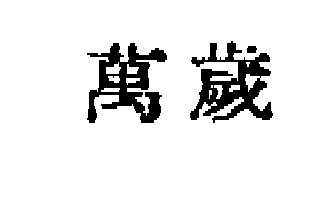
\includegraphics[width=2.6402in,height=0.9374in]{A2-img002.png} \par}

\bigskip
\end{document}
